\documentclass[times, utf8, seminar]{fer}
\usepackage{booktabs}
\usepackage{verbatim}
\usepackage{listings}
\usepackage{graphicx}
\usepackage{natbib}
\usepackage{subcaption}
\usepackage{color}
\usepackage{amssymb}
\usepackage{dsfont}

\begin{document}

% TODO: Navedite naslov rada.
\title{The Transformer Architecture: Facilitating Effective Pretraining and Task Adaptation}

% TODO: Navedite vaše ime i prezime.
\author{Antonio Lukić}

% TODO: Navedite ime i prezime mentora.
\mentor{prof.~dr.~sc.~Jan Šnajder, mag.~ing.~David Dukić}

\maketitle

\tableofcontents

\chapter{Introduction}
A good portion of the population has heard, encountered, or used ChatGPT or other applications powered by large language models. The field of Natural Language Processing (NLP) went through an intense transformation in recent years, largely driven by the models based on transformer architecture. These models, such as BERT \citep{devlin2018bert} and GPT (Generative Pre-Training) \citep{radford2018improving} have left a mark on how we interact with language technologies. From the appearance of these models, they have transformed society by automating tasks and enhancing communication and content creation. It has also raised concerns about job displacement, misinformation, and ethics. Understanding how to effectively employ these language technologies is equally important. To address these challenges, it is important to analyze where these models came from and what their direction of development is. Foundational papers, such as "Attention Is All You Need" \citep{vaswani2017attention}, laid the groundwork for the Transformer architecture, enabling further advancements.


Throughout this work, I will analyze five papers associated with Transformer model architecture. The analysis will start with foundational papers and then some of the contemporary developments in the NLP field, focusing on the effective pretraining and adaptation capabilities of the Transformer architecture. I will study different approaches presented in the papers and analyze their results. Finally, I will formulate conclusions about the current state of the field and what could hypothetically be my contribution to further development.

\chapter{Attention Is All You Need \citep{vaswani2017attention}}
This paper proposes a novel neural network architecture, the Transformer,
based for the most part on the attention mechanisms, dispensing with recurrence and convolutions entirely \citep{vaswani2017attention}. It describes well-thought-out Transformer architecture. Additionally, the authors have presented the results of the English-to-German, English-to-French translation task, and English constituency parsing task. The motivation for using only self-attention has three reasons: computational complexity per layer, amount of computation that can be parallelized, and path length between long-range dependencies in the network.


The previous works used Recurrent neural networks \citep{chung2014empirical, bahdanau2014neural} as model architecture and were state-of-the-art. However, these models divide the computation into sequential components. This sequential computation precludes parallelization and is sensitive to order and distance between words. On the other hand, this paper shows that the Transformer can model the dependencies regardless of the order and can be made parallelizable.


The Transformer architecture can be seen in Figure \ref{fig:transformer_architecture}.
\begin{figure}[htb]
\centering
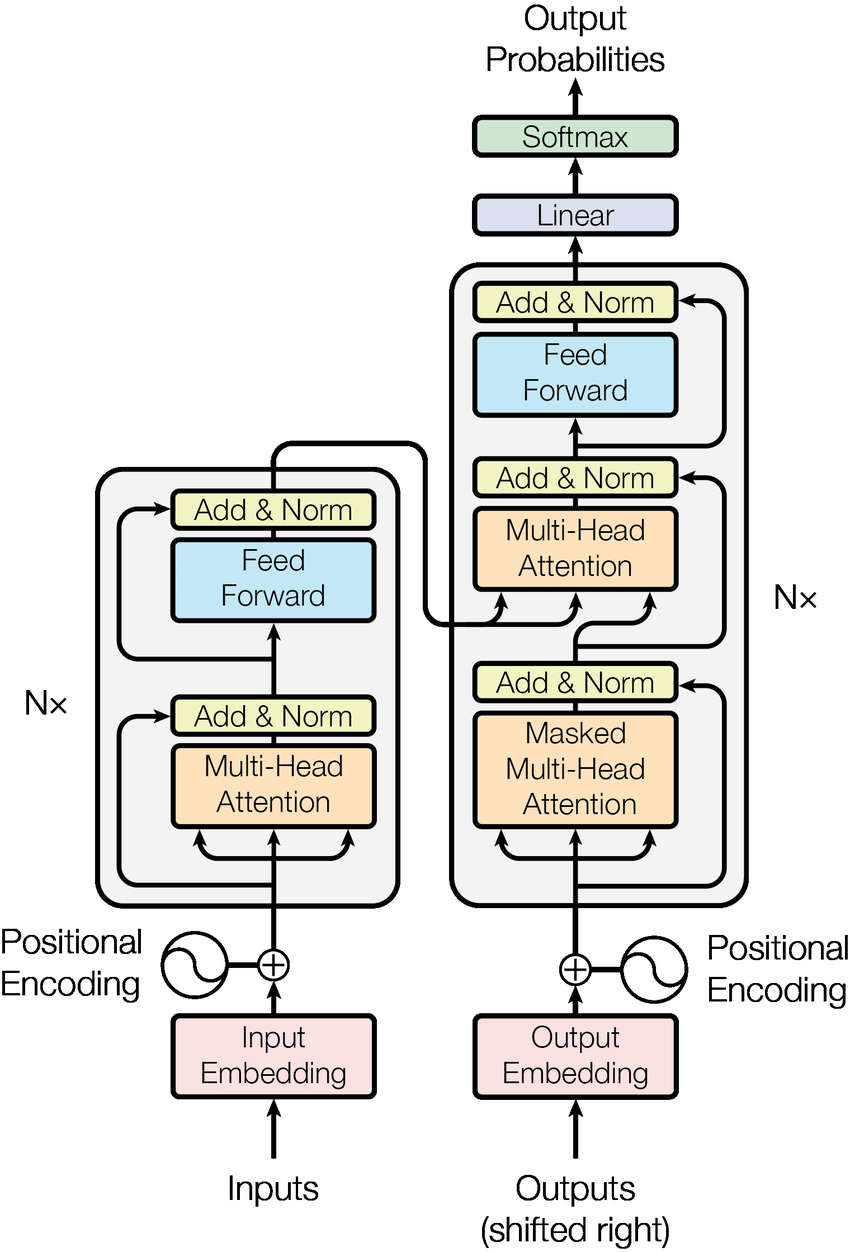
\includegraphics[width=5cm]{img/transformer_architecture.png}
\caption{The Transformer - model architecture}
\label{fig:transformer_architecture}
\end{figure}
It consists of encoder and decoder stacks. The encoder stack consists of layers. Each layer has two sublayers. The first sublayer is a multi-head self-attention mechanism, and the other is a feed-forward network. Each sublayer has a layer of normalization, so the output of a sublayer is LayerNorm(x + Sublayer(x)). The decoder stack is similar to the encoder, but it has three sublayers. The additional middle sublayer is the self-attention mechanism over the output of the encoder stack. The Transformer has auto-regression property.  It means that during training, each position in the input sequence can only attend to positions before it, preventing information flow from future positions. To ensure that, these sublayer inputs of the self-attention are modified to make the self-attention equal to 0. Words that enter the model are turned into vectors with embeddings, and then the positional encodings are added to those vectors. The self-attention is defined as $softmax \left(\dfrac{QK^T}{\sqrt{d_k}}\right)V$, where Q is the query matrix, K key matrix, V value matrix and $d_k$ is the number of columns in matrix K. Multi-head attention differs in a way that these matrices are multiplied by projection matrices and the attention of each head is concatenated into one multi-head. Finally, to get the output, apply a linear and softmax layer.


The datasets used for translation tasks were the WMT 2014 English-German dataset and the WMT 2014 English-French dataset. English-German dataset consisted of about $4.5$M sentence pairs while the English-French consisted of $36$M sentence pairs. For English Constituency Parsing, the Wall Street Journal (WSJ) portion of the
Penn Treebank \citep{marcus1993building} consisting of about 40K training sentences was used.


The results in the paper show that Transformer is state-of-the-art by achieving the highest BLEU score \citep{papineni2002bleu} on both translation tasks and at minimal training cost. On the English constituency task, the Transformer was only beaten by Recurrent Neural Network Grammar \citep{kuncoro2016recurrent}.


From my perspective, I think that the paper is well-structured and well-researched. Moreover, the authors released the code along with the paper, which contributes to the trustworthiness of their work. On the other hand, for a person who encounters an attention mechanism for the first time, hyperparameter choices such as positional encoding and the meaning of Q, K, and V matrices could be explained in more detail. In conclusion, the paper showed the crucial role of attention mechanisms but could have placed a bigger focus on simplifying the architectural choices and giving more intuitive explanations.


\chapter{Improving Language Understanding by Generative Pre-Training \citep{radford2018improving}}
The paper uses the Transformer architecture and represents a continuation of the previous paper. This paper emphasizes natural language understanding, highlighting tasks like textual entailment, question answering, semantic similarity, and document classification. The idea is to first do \emph{generative auto-regressive pre-training} on a diverse corpus of unlabeled data and then perform \emph{discriminative fine-tuning} on each specific task with labeled data \citep{radford2018improving}. The motivation for this approach is that plentiful unlabeled data is available but rarely labeled data that is expensive and time-consuming to obtain.

In the related work for semi-supervised learning for NLP, some approaches used unlabeled data to compute word-level statistics, which are then used as features in a supervised model \citep{liang2005semi}. This paper focuses on obtaining higher-than-word-level semantics. Moreover, some similar works involve pre-training a neural network using language modeling objectives and then fine-tuning it on a target task with supervision. However, those works cannot capture long-range relationships or use hidden representations from a pre-trained model \citep{peters2017semi}, which requires a significant amount of change to the model architecture depending on a task. Furthermore, this paper uses an auxiliary training objective which has been shown to enhance performance \citep{rei2017semi}.


The authors of the paper use the Transformer decoder as the model to be able to generate text. For unsupervised pre-training with an unlabeled corpus of tokens $\mathcal{U} = \{u_1,...,u_n\}$, the authors aim to maximise the likelihood:
\begin{equation}
L_1(\mathcal{U}) = \sum_i  log P \left(u_i|u_{i-k},...,u_{i-1};\Theta\right)
\label{eq:unsupervised_pretraining}
\end{equation}
where k is the window size and $\Theta$ are the parameters of the neural network which models the probability P. After unsupervised pre-training, the next step involves supervised fine-tuning. It assumes the availability of a labeled dataset $\mathcal{C} = {x_1, ..., x_n}$ with corresponding labels $y$, aiming to maximize:
\begin{equation}
L_2(\mathcal{C}) = \sum_{(x, y)}  log P \left(x_i|x_{i-k},...,x_{i-1}\right).
\label{eq:supervised_finetuning}
\end{equation}
Additionally, the axillary objective has been examined: $L_3(\mathcal{C}) = L_2(\mathcal{C}) + \lambda * L_1(\mathcal{C})$.

The paper outlines a two-step approach, emphasizing that the model can be fine-tuned for textual entailment, similarity, and question answering with minimal input modification. Specifically for classification, the authors propose direct fine-tuning by adding only randomly initialized start and end tokens to the original input.


Unsupervised pre-training is done on the BooksCorpus dataset \citep{zhu2015aligning} which contains over $7000$ unique unpublished books. For each task, various datasets are used for which I am going to mention only a few:
\begin{description}
    \item [\textbf{Natural language inference}:] SNLI\citep{bowman2015large}, RTE\citep{bentivogli2009fifth}
    \item [\textbf{Question answering}:] RACE\citep{lai2017race}, Story Cloze\citep{mostafazadeh2017lsdsem}
    \item [\textbf{Sentence similarity}:] MRPC\citep{dolan2005automatically}, QQP\citep{quoraquestion}
    \item [\textbf{Classification}:] Stanford Sentiment Treebank-2\citep{socher2013recursive}, CoLA \citep{warstadt2018corpus}
\end{description}


The results provided show that this approach outperforms all compared models on all datasets on question answering and commonsense reasoning. For classification and semantic similarity, a model exists that performs better only on CoLa and a model exists that performs better only on MRPC. It achieves new state-of-the-art results. The authors have also done ablation studies that are worth mentioning. It shows that the $L_3$ objective where $L_1$ is the auxiliary objective, is crucial for big datasets. Additionally, the authors observe a 5.6 average score drop when using the LSTM instead of the Transformer. Finally, when the model is trained directly without pre-training, the results are significantly worse, showing a decline of $14.8\%$.


From my perspective, the paper provided an effective way of transfer learning, allowing the model to learn general language representations before adapting to specific tasks. However, while the methods and objective functions are well described, there are some inconsistencies between the figure of input transformations for specific tasks and what is described in the text. Without the code and enough resources, it's hard to replicate the results reliably. The methods presented in this paper are well-supported by experimental results, thereby establishing a new advancement. The paper introduces the first significant pre-trained decoder transformer. 

\chapter{BERT: Pre-training of Deep Bidirectional Transformers for Language Understanding \citep{devlin2018bert}}
This paper proposes a new language model called BERT, which stands for Bidirectional Encoder Representations from Transformers. The novel model is designed to pre-train deep bidirectional representations from the unlabeled text by joint conditioning on both the left and right context in all layers \citep{devlin2018bert}. The motivation is that unidirectional language models can only attend previous tokens and thereby are limited in making better pre-trained representations and fine-tuning for contextual natural language understanding.


In the related work, feature-based approaches such as ELMo \citep{peters-etal-2018-deep} need task-specific architecture and the representation is a linear combination of the hidden states from both the forward and backward LSTMs as context whereas BERT considers all positions in the sequence simultaneously capturing both left and right contexts during training. Moreover, fine-tuning approaches such as \citep{radford2018improving}, benefit from not learning the representations from scratch.


As in the previous paper, BERT also uses a two-step approach of pretraining over unlabeled data and then fine-tuning for each specific task. This process is called transfer learning. BERT's architecture is a multi-layer bidirectional Transformer encoder based on the encoder part of the transformer model presented in the paper \citep{vaswani2017attention}. The input could be one or more sentences but the BERT packs them all into one sequence unlike \citep{radford2018improving}. The authors used WordPiece embeddings \citep{wu2016google}. The first token of every sequence is a special token [CLS]. It is used to aggregate sequence representation for classification tasks. To separate the sentences the authors used the [SEP] token. The input is the sum of 3 embeddings. Learned positional embedding in a sequence, segment embeddings that annotate from which sentence they are and token embeddings.


Unlike the previous models, BERT is pre-trained using two unsupervised tasks. \textbf{Masked language modeling} (MLM) is masking the input tokens for the model to guess the masked tokens. The authors mask $15\%$ of the token input. Of this, $80\%$ are replaced with [MASK] token, $10\%$ with a random token and $10\%$ is unchanged to avoid a mismatch between pre-training and fine-tuning. \textbf{Next Sentence Prediction} (NSP) is used to enhance understanding of sentence relationships. BERT uses a binarized next sentence prediction task, where pairs of sentences are selected, and $50\%$ of the time, the second sentence is the actual next sentence (IsNext), while $50\%$ it's a random sentence (NotNext). Pre-training is done on the already mentioned bookcorpus \citep{zhu2015aligning} and English Wikipedia. Fine-tuning BERT for tasks is simplified through a straightforward adaptation, achieved by swapping out task-specific inputs and outputs.


The datasets used for evaluation are various. Firstly, the GLUE benchmark covers all datasets used in \citep{radford2018improving}. The results show an improvement on all tasks over OpenAI GPT, setting new state-of-the-art results. Moreover, a collection of question/answer pairs SQuAD 1.1\citep{rajpurkar2016squad} and SQuAD 2.0 were analyzed. In both datasets, BERT was again a new state-of-the-art system but on SQuAD 2.0, it did not outperform humans. Furthermore, the SWAG dataset \citep{zellers2018swag}, a collection of selecting the most plausible continuation among four choices, was analyzed. BERT here also sets state-of-the-art results.


Additionally, the authors conducted ablation studies. They showed that removing NSP significantly hurts QNLI, MNLI, and SQUAD 1.1. Moreover, MLM without NSP performs better than the left-to-right context model without NSP.


From my perspective, the paper presented new and original research. The paper introduced new architecture, thus new pre-training unsupervised tasks and new datasets for analysis. However, while intriguing these novelties are, I struggled to understand how BERT processes tokens for evaluating some datasets. Furthermore, the intuition behind pre-training unsupervised tasks could be more clarified. Additionally, it would have been helpful if the paper compared BERT more directly to the OpenAI GPT model \citep{radford2018improving}. This would give a clearer picture of how BERT improves upon the earlier model and what makes it stand out. Overall, BERT provides a step further in NLP with detailed results on various datasets. The paper was composed as a response to the \citep{radford2018improving} study, surpassing the OpenAI GPT model and thereby establishing new state-of-the-art results.

\chapter{Don’t Stop Pretraining: Adapt Language Models to Domains and Tasks \citep{gururangan2020don}}
This paper analyses whether it is still helpful to adapt the model, after pre-training to a domain or target task. The motivation is to investigate whether the latest large pre-trained models have consistent performance across diverse domains, tasks and datasets. Specifically, the model that is used is RoBERTa \citep{liu2019roberta}.


The prior works have shown the benefits of continued pre-training in the domain \citep{lee2020biobert}, but in contrast to this paper, they used one domain at a time and a smaller and less diverse corpus. Additionally, previous works have also shown the advantage of continued pretraining through \emph{task-adaptive pretraining} (TAPT) for improved end-task performance \citep{howard2018universal, phang2018sentence}. This paper additionally explores its comparison with \emph{domain-adaptive pretraining} (DAPT), examining their interaction in transferability to other tasks and multi-phase pretraining strategies.


The authors focused on four domains which are centered around genres and forums. Domains are biomedical (BIOMED) papers, computer science (CS) papers, news text from REALNEWS, and AMAZON reviews. The tasks they focused on were two classification tasks from each domain. Before conducting the additional pre-training, the authors compared the similarity between the four mentioned domains and the original domain of RoBERTa. Consequently, showing that original RoBERTa's domain is most similar to News and Reviews, therefore, the most benefits could get BIOMED and CS.


After training on all domains together and additionally on each domain separately, the authors show that loss only increases in News. Furthermore, the \emph{$F_1$} score across all tasks rises by $2\%$ on average except for one dataset from NEWS where it stays the same and for one dataset from CS where it has risen by $12.5\%$. The baseline model RoBERTa is not far behind. Additionally, when doing DAPT on the most dissimilar domain the \emph{$F_1$} score drops from the baseline for all except the CS domain. This goes to show that better performance is not obtained by simply exposure to more data regardless of the domain. The authors pointed out another interesting point of view that since domain overlapping in the datasets leads to unexpected positive transfer, training on unconventional domains beyond conventional boundaries could yield better results for DAPT.


Furthermore, the paper shows that training on the task data, a narrowly defined subset of the domain that is more relevant to the task, is beneficial. TAPT raises \emph{$F_1$} score on all domain tasks. DAPT is more resource-intensive but TAPT manages to keep up. Finally, when applying DAPT on RoBERTa and then TAPT yields the best results on tasks. Another analysis for TAPT is to pre-train on one task and then fine-tune on the other task in the same domain. The paper shows a clear drop in performance across all tasks. It shows that data distributions within the domain of tasks differ and that adapting to a broad domain is not sufficient.


The last set of analyses deals with augmenting training data for TAPT for BIOMED and CS domains. It is the same principle as TAPT but on a larger dataset curated by humans or it is automated. DAPT + human curated-TAPT outperforms DAPT + TAPT and only human curated-TAPT on these tasks suggests that curating large amounts of data is beneficial. For automated curated-TAPT, the authors use VAMPIRE \citep{gururangan2019variational} bag-of-words language model. The goal is to find task-relevant data from the domain by embedding text from task and domain in a shared space and then finding the candidates from the domain by using queries and VAMPIRE from task data. The candidates were chosen by the \emph{k}-NN algorithm or randomly. The paper shows that both types of candidate selection are better than TAPT but worse than DAPT.


This paper has had some creative and interesting analysis. The paper is well-written and I was fascinated by the combination of the usage of DAPT and TAPT as well as both human-curated and automated methods for expanding the data. On the other hand, the paper could use a more detailed discussion of the dataset's biases and representativeness. The choice of hyperparameters or the choice of specific architectures such as for VAMPIRE is not explored enough in my opinion. The analysis of the combination of DAPT and TAPT shows improved results but could be further investigated on the trade-offs between domain diversity and task relevance. In conclusion, the work provides valuable contributions to the understanding of continued pretraining strategies, domain adaptation, and task-specific adaptability.

\chapter{TaCL: Improving BERT Pre-training with Token-aware Contrastive Learning \citep{su2021tacl}}
This paper proposes a continual novel and effective pre-training approach called TaCL (Token-aware Contrastive Learning). TaCL pre-training is unsupervised and requires no additional data. The motivation for this is that pre-trained MLMs like BERT \citep{devlin2018bert} output an anisotropic distribution of token representations that live in a narrow subset of the entire representation space. This kind of token representation is not ideal for discriminative tasks.


Prior work showed the benefits of continual pre-training \citep{gururangan2020don}. Furthermore, related works used sentence-level contrastive learning with sentence-level embeddings \citep{giorgi2020declutr} but have not been tested on improving general-purpose token representations and have no evidence that they will work on more complex datasets such as SQuAD \citep{rajpurkar2016squad}.

\begin{figure}[htb]
\centering
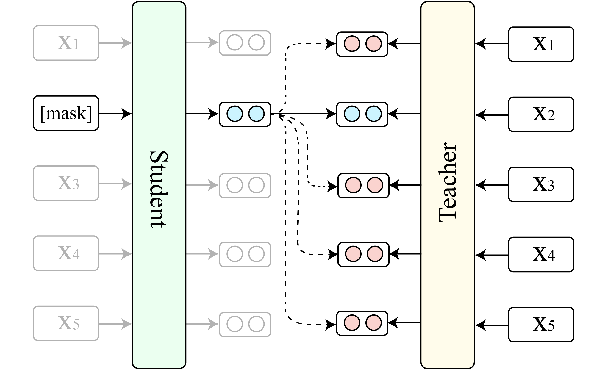
\includegraphics[width=7cm]{img/tacl_objective.png}
\caption{TaCL objective}
\label{fig:tacl_objective}
\end{figure}

The authors use two BERT models in their research. One is called the student and the other one is called the teacher and they are the same pre-trained BERT model. The concept of learning is to freeze the teacher and optimize the student model. The student model is optimized with the original BERT MLM and NSP objective \citep{devlin2018bert} and a new TaCL objective. TaCL's objective, shown in Figure \ref{fig:tacl_objective}, is to contrast the masked token from the student to the unmasked same token from the teacher by getting closer to the teacher's unmasked token and getting further from the student's reference tokens in the same sequence. The ith token in the input sequence is represented by $x_i$, $\tilde{x_i}$ is the masked input token, $h_i$ is the ith output token of the teacher and $\tilde{h}_i$ is the ith token output of the student. The TaCL with the described objective is then:
\begin{equation}
\mathcal{L}_{TaCL} = -\sum\limits^n\limits_{i=1} \mathds{1}(\tilde{x}_i)log\frac{exp(sim(\tilde{h}_i, h_h))/\tau}{\sum^n_{j=1}exp(sim(\tilde{h}_i, h_j)/\tau)}
\label{eq:tacl_objective}
\end{equation}
where $\mathds{1}$ is the indicator function being 1 when $\tilde{x}_i$ is a masked token, the \emph{sim} is cosine similarity and $\tau$ is a hyperparameter. Another measurement used in this paper is \emph{self-similarity} which is the sum of all cosine similarities of each token to all other tokens in the model output. The lower the self-similarity the more discriminative the tokens are. Since this model operates on the improvement of token-level representations, it can be quite beneficial for token classification tasks.


The datasets used for the English benchmark are the same datasets used in \citep{devlin2018bert} to be comparable to the BERT model. For the Chinese benchmark, the authors evaluate the model in tasks on various datasets. Naming only a few, for named entity recognition (NER) \citep{weischedel2011ontonotes} \citep{levow2006third} and for Chinese word segmentation (CWS) \citep{emerson2005second}.


TaCL outperforms BERT on the majority of English datasets, showing improvements ranging from $0.5$ to $2$ in the $F_1$ score. However, its performance is slightly worse on QNLI and CoLA. For Chinese datasets, TaCL performs better than baseline BERT on all datasets having an improvement from $0.5$ to $2$. Ablation studies have also been made on the SQuAD 1.1 and SQuAD 2.0, showing that training on sentence-level contrastive objective as proposed by \citep{liu2021fast}, is worse by $0.6$ and $1$. Moreover, training with only the TaCL objective shows that the model suffers a loss of $0.3$ and $0.4$. Furthermore, results of self-similarity on SQuAD show that by all layers, the self-similarity in baseline BERT is higher than training with TaCl objective except in the last output layer. In the last layer of TaCL, the self-similarity significantly drops which shows that the learned representations are more discriminative.


From my perspective, this paper provides a good view of the limitations of token representations from BERT. It was very intriguing to see that without any need for additional data, the model could be even more improved. The authors gave a clear explanation of methods, objectives, and what their goal was. However, the paper did not conduct hyperparameter tuning. I would have liked to see a deeper analysis of why the self-similarity is lower only in the final layer. Additionally, the detailed analysis of self-similarity and ablation studies is done only on SQuAD, which could show only this approach's benefits. To sum up, TaCL has the potential to make token representations better, but it needs further exploration.

\chapter{Conclusion}
All the papers throughout this work were intriguing. The papers provided how rapidly the architecture and pre-training approaches have been evolving over the years. I was especially impressed by the variety and cleverness of the approaches, such as DAPT, TAPT, and token-aware contrastive learning. Moreover, I liked how token-aware contrastive learning was made without the need for additional data. From the appearance, the Transformers are the state-of-the-art model in the field of NLP. Today, the two-step approach of pre-training and fine-tuning is a typical learning paradigm. Further development could explore more advanced pre-training techniques regarding biases of the domain. Hypothetically, my contribution could involve developing some domain-specific pre-training methods, ensuring that models are performing various tasks within a specific domain. A step in this direction might involve experimenting with transfer learning approaches across related domains. To be able to contribute I would need a much deeper understanding of domain adaptation and transfer learning. Another contribution could be linked to model interpretability which could explain model decisions with higher granularity.

\bibliography{literatura}
\bibliographystyle{fer}

\end{document}
